\documentclass{standalone}
\usepackage{tikz}
\usetikzlibrary{patterns, positioning}

\begin{document}
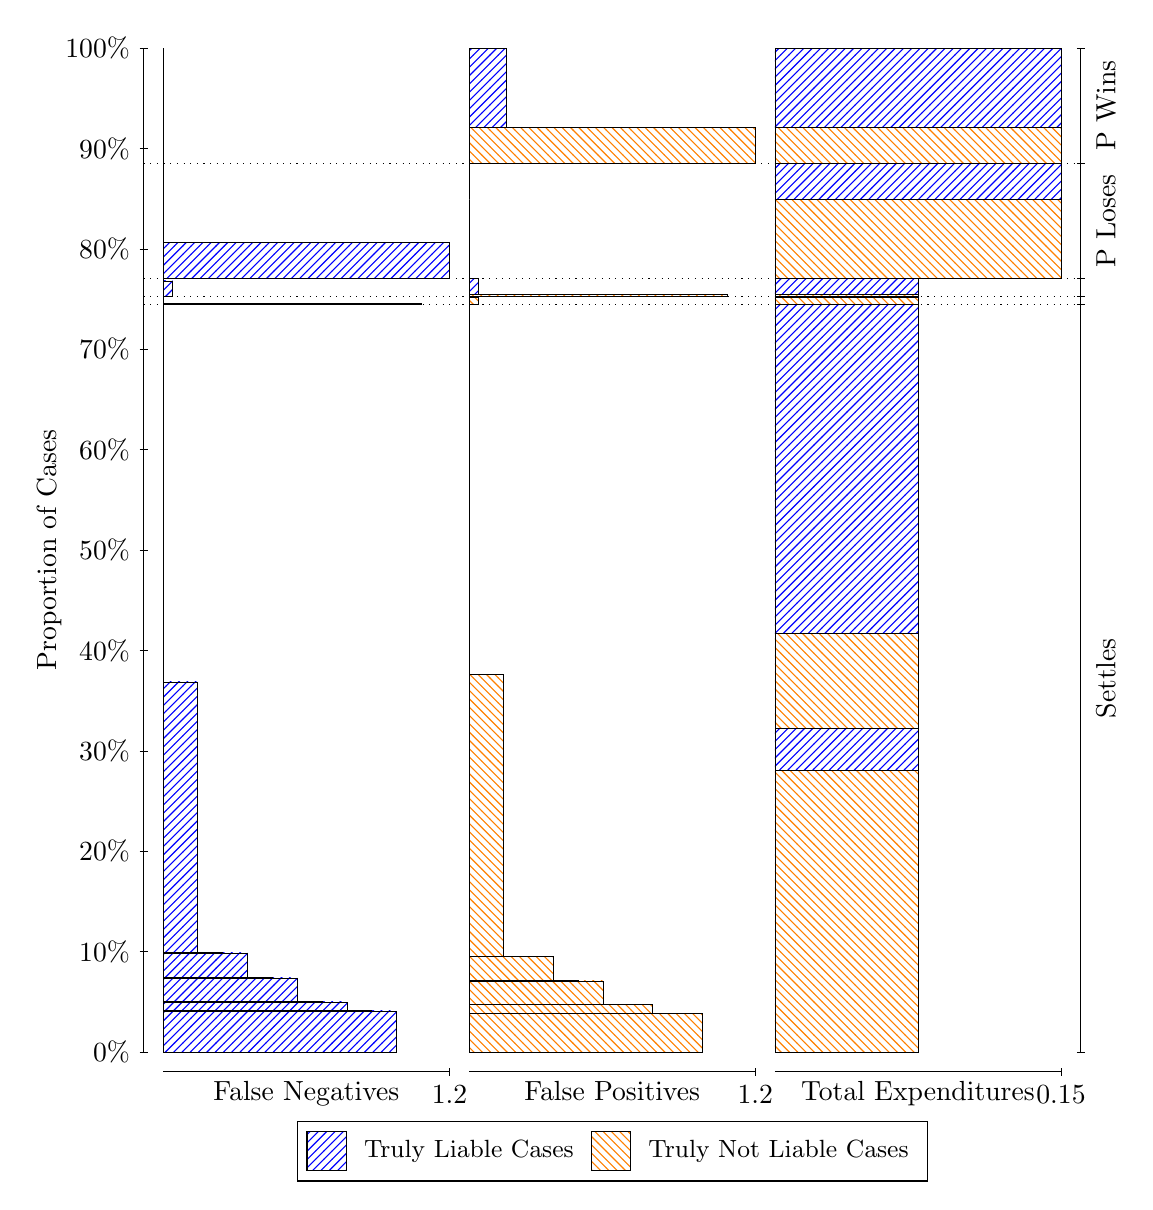
\begin{tikzpicture}
\draw[black, very thin] (1.5,1.75) -- (1.5,14.5);
\node[rotate=90, anchor=center] at (0.3, 8.125) {Proportion of Cases};
\draw[black, very thin] (1.45,1.75) -- (1.55,1.75);
\node[anchor=east] at (1.45, 1.75) {0\%};
\draw[black, very thin] (1.45,3.025) -- (1.55,3.025);
\node[anchor=east] at (1.45, 3.025) {10\%};
\draw[black, very thin] (1.45,4.3) -- (1.55,4.3);
\node[anchor=east] at (1.45, 4.3) {20\%};
\draw[black, very thin] (1.45,5.575) -- (1.55,5.575);
\node[anchor=east] at (1.45, 5.575) {30\%};
\draw[black, very thin] (1.45,6.85) -- (1.55,6.85);
\node[anchor=east] at (1.45, 6.85) {40\%};
\draw[black, very thin] (1.45,8.125) -- (1.55,8.125);
\node[anchor=east] at (1.45, 8.125) {50\%};
\draw[black, very thin] (1.45,9.4) -- (1.55,9.4);
\node[anchor=east] at (1.45, 9.4) {60\%};
\draw[black, very thin] (1.45,10.675) -- (1.55,10.675);
\node[anchor=east] at (1.45, 10.675) {70\%};
\draw[black, very thin] (1.45,11.95) -- (1.55,11.95);
\node[anchor=east] at (1.45, 11.95) {80\%};
\draw[black, very thin] (1.45,13.225) -- (1.55,13.225);
\node[anchor=east] at (1.45, 13.225) {90\%};
\draw[black, very thin] (1.45,14.5) -- (1.55,14.5);
\node[anchor=east] at (1.45, 14.5) {100\%};

\draw[black, very thin] (13.4,1.75) -- (13.4,14.5);
\draw[black, very thin] (13.35,1.75) -- (13.45,1.75);
\node[anchor=west] at (13.35, 1.75) {};
\draw[black, very thin] (13.35,11.244) -- (13.45,11.244);
\node[anchor=west] at (13.35, 11.244) {};
\draw[black, very thin] (13.35,11.341) -- (13.45,11.341);
\node[anchor=west] at (13.35, 11.341) {};
\draw[black, very thin] (13.35,11.575) -- (13.45,11.575);
\node[anchor=west] at (13.35, 11.575) {};
\draw[black, very thin] (13.35,13.037) -- (13.45,13.037);
\node[anchor=west] at (13.35, 13.037) {};
\draw[black, very thin] (13.35,14.5) -- (13.45,14.5);
\node[anchor=west] at (13.35, 14.5) {};

\draw[black, very thin, pattern color=blue, pattern=north east lines] (1.75,1.75) rectangle (4.712,2.2724);
\draw[black, very thin, pattern color=blue, pattern=north east lines] (1.75,2.2724) rectangle (4.396,2.2756);
\draw[black, very thin, pattern color=blue, pattern=north east lines] (1.75,2.2756) rectangle (4.0801,2.3854);
\draw[black, very thin, pattern color=blue, pattern=north east lines] (1.75,2.3854) rectangle (3.7641,2.389);
\draw[black, very thin, pattern color=blue, pattern=north east lines] (1.75,2.389) rectangle (3.4482,2.6898);
\draw[black, very thin, pattern color=blue, pattern=north east lines] (1.75,2.6898) rectangle (3.1322,2.6948);
\draw[black, very thin, pattern color=blue, pattern=north east lines] (1.75,2.6948) rectangle (2.8163,3.0097);
\draw[black, very thin, pattern color=blue, pattern=north east lines] (1.75,3.0097) rectangle (2.5004,3.0101);
\draw[black, very thin, pattern color=blue, pattern=north east lines] (1.75,3.0101) rectangle (2.1844,6.4513);
\draw[black, very thin, pattern color=orange, pattern=north west lines] (1.75,6.4513) rectangle (1.75,11.244);
\draw[black, very thin, pattern color=blue, pattern=north east lines] (1.75,11.244) rectangle (5.0279,11.253);
\draw[black, very thin, pattern color=orange, pattern=north west lines] (1.75,11.253) rectangle (1.75,11.341);
\draw[black, very thin, pattern color=blue, pattern=north east lines] (1.75,11.341) rectangle (1.8685,11.544);
\draw[black, very thin, pattern color=orange, pattern=north west lines] (1.75,11.544) rectangle (1.75,11.575);
\draw[black, very thin, pattern color=blue, pattern=north east lines] (1.75,11.575) rectangle (5.3833,12.034);
\draw[black, very thin, pattern color=orange, pattern=north west lines] (1.75,12.034) rectangle (1.75,13.037);
\draw[black, very thin, pattern color=orange, pattern=north west lines] (1.75,13.037) rectangle (1.75,13.497);
\draw[black, very thin, pattern color=blue, pattern=north east lines] (1.75,13.497) rectangle (1.75,14.5);
\draw[black, very thin, pattern color=orange, pattern=north west lines] (5.6333,1.75) rectangle (8.5953,2.2413);
\draw[black, very thin, pattern color=orange, pattern=north west lines] (5.6333,2.2413) rectangle (8.2793,2.242);
\draw[black, very thin, pattern color=orange, pattern=north west lines] (5.6333,2.242) rectangle (7.9634,2.353);
\draw[black, very thin, pattern color=orange, pattern=north west lines] (5.6333,2.353) rectangle (7.6475,2.3554);
\draw[black, very thin, pattern color=orange, pattern=north west lines] (5.6333,2.3554) rectangle (7.3315,2.6527);
\draw[black, very thin, pattern color=orange, pattern=north west lines] (5.6333,2.6527) rectangle (7.0156,2.6542);
\draw[black, very thin, pattern color=orange, pattern=north west lines] (5.6333,2.6542) rectangle (7.0156,2.6575);
\draw[black, very thin, pattern color=orange, pattern=north west lines] (5.6333,2.6575) rectangle (6.6996,2.9623);
\draw[black, very thin, pattern color=orange, pattern=north west lines] (5.6333,2.9623) rectangle (6.3837,2.9656);
\draw[black, very thin, pattern color=orange, pattern=north west lines] (5.6333,2.9656) rectangle (6.0678,6.5423);
\draw[black, very thin, pattern color=blue, pattern=north east lines] (5.6333,6.5423) rectangle (5.6333,11.244);
\draw[black, very thin, pattern color=orange, pattern=north west lines] (5.6333,11.244) rectangle (5.7518,11.332);
\draw[black, very thin, pattern color=blue, pattern=north east lines] (5.6333,11.332) rectangle (5.6333,11.341);
\draw[black, very thin, pattern color=orange, pattern=north west lines] (5.6333,11.341) rectangle (8.9112,11.373);
\draw[black, very thin, pattern color=blue, pattern=north east lines] (5.6333,11.373) rectangle (5.7518,11.575);
\draw[black, very thin, pattern color=orange, pattern=north west lines] (5.6333,11.575) rectangle (5.6333,12.578);
\draw[black, very thin, pattern color=blue, pattern=north east lines] (5.6333,12.578) rectangle (5.6333,13.037);
\draw[black, very thin, pattern color=orange, pattern=north west lines] (5.6333,13.037) rectangle (9.2667,13.497);
\draw[black, very thin, pattern color=blue, pattern=north east lines] (5.6333,13.497) rectangle (6.1072,14.5);
\draw[black, very thin, pattern color=orange, pattern=north west lines] (9.5167,1.75) rectangle (11.333,5.3299);
\draw[black, very thin, pattern color=blue, pattern=north east lines] (9.5167,5.3299) rectangle (11.333,5.8556);
\draw[black, very thin, pattern color=orange, pattern=north west lines] (9.5167,5.8556) rectangle (11.333,7.0679);
\draw[black, very thin, pattern color=blue, pattern=north east lines] (9.5167,7.0679) rectangle (11.333,11.244);
\draw[black, very thin, pattern color=orange, pattern=north west lines] (9.5167,11.244) rectangle (11.333,11.332);
\draw[black, very thin, pattern color=blue, pattern=north east lines] (9.5167,11.332) rectangle (11.333,11.341);
\draw[black, very thin, pattern color=orange, pattern=north west lines] (9.5167,11.341) rectangle (11.333,11.373);
\draw[black, very thin, pattern color=blue, pattern=north east lines] (9.5167,11.373) rectangle (11.333,11.575);
\draw[black, very thin, pattern color=orange, pattern=north west lines] (9.5167,11.575) rectangle (13.15,12.578);
\draw[black, very thin, pattern color=blue, pattern=north east lines] (9.5167,12.578) rectangle (13.15,13.037);
\draw[black, very thin, pattern color=orange, pattern=north west lines] (9.5167,13.037) rectangle (13.15,13.497);
\draw[black, very thin, pattern color=blue, pattern=north east lines] (9.5167,13.497) rectangle (13.15,14.5);
\draw[black, dotted] (1.5,11.244) -- (13.4,11.244);
\draw[black, dotted] (1.5,11.341) -- (13.4,11.341);
\draw[black, dotted] (1.5,11.575) -- (13.4,11.575);
\draw[black, dotted] (1.5,13.037) -- (13.4,13.037);
\draw[black, very thin] (1.75,1.5) -- (5.3833,1.5);
\node[anchor=north] at (3.5667, 1.5) {False Negatives};
\draw[black, very thin] (5.3833,1.45) -- (5.3833,1.55);
\node[anchor=north] at (5.3833, 1.45) {1.2};

\draw[black, very thin] (5.6333,1.5) -- (9.2667,1.5);
\node[anchor=north] at (7.45, 1.5) {False Positives};
\draw[black, very thin] (9.2667,1.45) -- (9.2667,1.55);
\node[anchor=north] at (9.2667, 1.45) {1.2};

\draw[black, very thin] (9.5167,1.5) -- (13.15,1.5);
\node[anchor=north] at (11.333, 1.5) {Total Expenditures};
\draw[black, very thin] (13.15,1.45) -- (13.15,1.55);
\node[anchor=north] at (13.15, 1.45) {0.15};

\node[black, centered, rotate=90] at (13.72, 6.4968) {Settles};


\node[black, centered, rotate=90] at (13.72, 12.306) {P Loses};
\node[black, centered, rotate=90] at (13.72, 13.769) {P Wins};

\draw (7.449999999999999,1.5) node[draw=none] (baseCoordinate) {};
\begin{scope}[align=center]
        \matrix[scale=0.5, draw=black, below=0.5cm of baseCoordinate, nodes={draw}, column sep=0.1cm]{
            \node[rectangle, draw, minimum width=0.5cm, minimum height=0.5cm, pattern=north east lines, pattern color=blue] {}; &
            \node[draw=none, font=\small] (B) {Truly Liable Cases}; &
            \node[rectangle, draw, minimum width=0.5cm, minimum height=0.5cm, pattern=north west lines, pattern color=orange] {}; &
            \node[draw=none, font=\small] (B) {Truly Not Liable Cases}; \\
            };
\end{scope}

\end{tikzpicture}
\end{document}